
% Template for Elsevier CRC journal article
% version 1.2 dated 09 May 2011

% This file (c) 2009-2011 Elsevier Ltd.  Modifications may be freely made,
% provided the edited file is saved under a different name

% This file contains modifications for Procedia Computer Science
% but may easily be adapted to other journals

% Changes since version 1.1
% - added "procedia" option compliant with ecrc.sty version 1.2a
%   (makes the layout approximately the same as the Word CRC template)
% - added example for generating copyright line in abstract

%-----------------------------------------------------------------------------------

%% This template uses the elsarticle.cls document class and the extension package ecrc.sty
%% For full documentation on usage of elsarticle.cls, consult the documentation "elsdoc.pdf"
%% Further resources available at http://www.elsevier.com/latex

%-----------------------------------------------------------------------------------

%%%%%%%%%%%%%%%%%%%%%%%%%%%%%%%%%%%%%%%%%%%%%%%%%%%%%%%%%%%%%%
%%%%%%%%%%%%%%%%%%%%%%%%%%%%%%%%%%%%%%%%%%%%%%%%%%%%%%%%%%%%%%
%%                                                          %%
%% Important note on usage                                  %%
%% -----------------------                                  %%
%% This file should normally be compiled with PDFLaTeX      %%
%% Using standard LaTeX should work but may produce clashes %%
%%                                                          %%
%%%%%%%%%%%%%%%%%%%%%%%%%%%%%%%%%%%%%%%%%%%%%%%%%%%%%%%%%%%%%%
%%%%%%%%%%%%%%%%%%%%%%%%%%%%%%%%%%%%%%%%%%%%%%%%%%%%%%%%%%%%%%

%% The '3p' and 'times' class options of elsarticle are used for Elsevier CRC
%% Add the 'procedia' option to approximate to the Word template
%\documentclass[3p,times,procedia]{elsarticle}
\documentclass[3p,times]{elsarticle}

%% The `ecrc' package must be called to make the CRC functionality available
\usepackage{ecrc}
\usepackage{graphicx}
\usepackage{subcaption}
\usepackage{amsmath}
%% The ecrc package defines commands needed for running heads and logos.
%% For running heads, you can set the journal name, the volume, the starting page and the authors

%% set the volume if you know. Otherwise `00'
\volume{00}

%% set the starting page if not 1
\firstpage{1}

%% Give the name of the journal
\journalname{Procedia Computer Science}

%% Give the author list to appear in the running head
%% Example \runauth{C.V. Radhakrishnan et al.}
\runauth{}

%% The choice of journal logo is determined by the \jid and \jnltitlelogo commands.
%% A user-supplied logo with the name <\jid>logo.pdf will be inserted if present.
%% e.g. if \jid{yspmi} the system will look for a file yspmilogo.pdf
%% Otherwise the content of \jnltitlelogo will be set between horizontal lines as a default logo

%% Give the abbreviation of the Journal.  Contact the journal editorial office if in any doubt
\jid{procs}

%% Give a short journal name for the dummy logo (if needed)
\jnltitlelogo{Procedia Computer Science}

%% Provide the copyright line to appear in the abstract
%% Usage:
%   \CopyrightLine[<text-before-year>]{<year>}{<restt-of-the-copyright-text>}
%   \CopyrightLine[Crown copyright]{2011}{Published by Elsevier Ltd.}
%   \CopyrightLine{2011}{Elsevier Ltd. All rights reserved}
\CopyrightLine{2011}{Published by Elsevier Ltd.}

%% Hereafter the template follows `elsarticle'.
%% For more details see the existing template files elsarticle-template-harv.tex and elsarticle-template-num.tex.

%% Elsevier CRC generally uses a numbered reference style
%% For this, the conventions of elsarticle-template-num.tex should be followed (included below)
%% If using BibTeX, use the style file elsarticle-num.bst

%% End of ecrc-specific commands
%%%%%%%%%%%%%%%%%%%%%%%%%%%%%%%%%%%%%%%%%%%%%%%%%%%%%%%%%%%%%%%%%%%%%%%%%%

%% The amssymb package provides various useful mathematical symbols
\usepackage{amssymb}
%% The amsthm package provides extended theorem environments
%% \usepackage{amsthm}

%% The lineno packages adds line numbers. Start line numbering with
%% \begin{linenumbers}, end it with \end{linenumbers}. Or switch it on
%% for the whole article with \linenumbers after \end{frontmatter}.
%% \usepackage{lineno}

%% natbib.sty is loaded by default. However, natbib options can be
%% provided with \biboptions{...} command. Following options are
%% valid:

%%   round  -  round parentheses are used (default)
%%   square -  square brackets are used   [option]
%%   curly  -  curly braces are used      {option}
%%   angle  -  angle brackets are used    <option>
%%   semicolon  -  multiple citations separated by semi-colon
%%   colon  - same as semicolon, an earlier confusion
%%   comma  -  separated by comma
%%   numbers-  selects numerical citations
%%   super  -  numerical citations as superscripts
%%   sort   -  sorts multiple citations according to order in ref. list
%%   sort&compress   -  like sort, but also compresses numerical citations
%%   compress - compresses without sorting
%%
%% \biboptions{comma,round}

% \biboptions{}

% if you have landscape tables
\usepackage[figuresright]{rotating}

% put your own definitions here:
%   \newcommand{\cZ}{\cal{Z}}
%   \newtheorem{def}{Definition}[section]
%   ...

% add words to TeX's hyphenation exception list
%\hyphenation{author another created financial paper re-commend-ed Post-Script}

% declarations for front matter

\begin{document}

\begin{frontmatter}

%% Title, authors and addresses

%% use the tnoteref command within \title for footnotes;
%% use the tnotetext command for the associated footnote;
%% use the fnref command within \author or \address for footnotes;
%% use the fntext command for the associated footnote;
%% use the corref command within \author for corresponding author footnotes;
%% use the cortext command for the associated footnote;
%% use the ead command for the email address,
%% and the form \ead[url] for the home page:
%%
%% \title{Title\tnoteref{label1}}
%% \tnotetext[label1]{}
%% \author{Name\corref{cor1}\fnref{label2}}
%% \ead{email address}
%% \ead[url]{home page}
%% \fntext[label2]{}
%% \cortext[cor1]{}
%% \address{Address\fnref{label3}}
%% \fntext[label3]{}

\dochead{}
%% Use \dochead if there is an article header, e.g. \dochead{Short communication}
%% \dochead can also be used to include a conference title, if directed by the editors
%% e.g. \dochead{17th International Conference on Dynamical Processes in Excited States of Solids}

\title{Surface Reconstruction From the Cross-Sections Based on FFD Matching}

%% use optional labels to link authors explicitly to addresses:
%% \author[label1,label2]{<author name>}
%% \address[label1]{<address>}
%% \address[label2]{<address>}

\author{}

\address{}

\begin{abstract}
%% Text of abstract
\end{abstract}

\begin{keyword}
%% keywords here, in the form: keyword \sep keyword

%% PACS codes here, in the form: \PACS code \sep code

%% MSC codes here, in the form: \MSC code \sep code
%% or \MSC[2008] code \sep code (2000 is the default)

\end{keyword}

\end{frontmatter}

%%
%% Start line numbering here if you want
%%
% \linenumbers

%% main text
\section{Introduction}
\label{section1}
%what is the problem
In the present work, a new framework has been developed to
reconstruct a object from a series of parallel planar
cross-sections(slices), each slice contains one or more contours, and
a 3-D surface will be obtained as a result.
%why is it interesting and important
%%the technique is very important for real applications

A high quality reconstruction is demanded by product designing, 3D-printing,
nondestructive inspection, medical imaging, or where need a visual
effect from the slices. Recently, with the improvements in data
acquisition and imagine techniques like MRI, CT and ultrasound
imaging, it's easy to get the slices which represent the object
precisely, which make the reconstruction from slices more practicably
 in many fields.
%%The request for
%%reconstruction objects from planar cross sections(also called slices)
%%arises in various applications, such as medical science,3D-Printing, and CAD/CAM
%why is it hard
%%simply introduction for 3D reconstruction based on 2D cross-sections

The procedure of 3D reconstruction based on the 2D cross-sections
usually consist of data acquisition, correspondence decision and
surface fitting. The correspondence problem can subdivide into two steps,
global correspondence and local correspondence. Global correspondence
decides the portions connection, and solves the branching
problem (many-to-many case), sometimes the branching problem is
considered as a independent problem Fig. \ref{fig:global}. And the local
correspondence(also called the tiling problem) decide how
to stitch the adjacent corresponding contours together,like
Fig. \ref{fig:local}. An automatic solution of the correspondence is
very difficult in its general form, since there is no constraints on
the adjacent slices, and it's very hard to extract the correspondence
from the adjacent dissimilar slices. The surface fitting step will
generate a smooth surface, and it is hot topic in computer
graphics.

%%this paper's overview
There has been a lot of previous research on the correspondence
problem, the most of them obtained the correspondence by advancing
rules or a set of constraints, it's really hard to deal with the
various difference between the adjacent slices.

This paper present a new frame work to do the reconstruction, all of which
works on the 2D planar cross sections. The correspondence problem is
solved by the free from deformation (FFD) matching, and the branching
problem is solved by the medial axis. Once corresponding points are
extracted, object surface can be quickly rendered by various classic algorithms. See more detail in Section \ref{section3}.
% algorithm's property
Our algorithm can solves the most general version of the problem, with
successive parallel slices, as well as the branching problem. The generated
surface is approximate to the contour's points, so is naturally
smooth.

The remainder of this paper is organized as follows. In section \ref{section2}, we
review previews work on reconstruction. In section \ref{section3}, we present in
detail our reconstruction framework. This includes the FFD matching,
branching problem and the detect of the capping region. In section
\ref{section4}, we show some example applications of our reconstruction framework, and analyze the accurate of the result.

\begin{figure}[ht]
\centering
\begin{subfigure}[b]{0.2\textwidth}
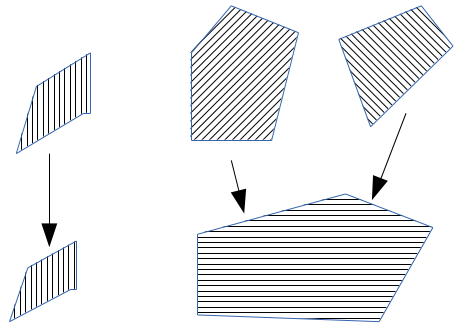
\includegraphics[width=\textwidth]{../picture/global.png}
\caption{global correspondence}
\label{fig:global}
\end{subfigure}%
~~~~~~~~~~~~~~~~~~~~~~~~~~~~~~~~~~~~~~~~~~~~%add desired spacing between images, blank line to force the
%subfigure to a new line
\begin{subfigure}[b]{0.2\textwidth}
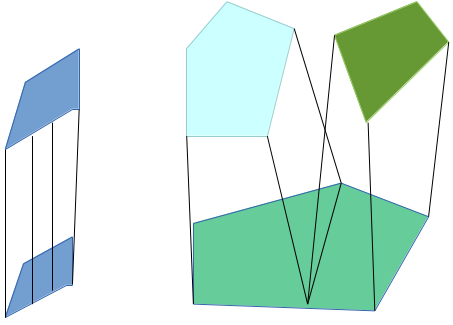
\includegraphics[width=\textwidth]{../picture/local.png}
\caption{local correspondence}
\label{fig:local}
\end{subfigure}

\caption{The correspondence decision}
\label{fig:the correspondence decision}
\end{figure}

\section{OVERVIEW OF PREVIOUS APPROACHES}
\label{section2}
Many solutions have proposed for the surface reconstruction problem,
some of them were suggested for the pure raster interpolation, the
interpolation produces one or more intermediate raster images, and
then extracted the surface from these raster images, like use the
level set method to obtain the surface. Cline et
al.\cite{cline_two_1988,lorensen_marching_1987} use the marching cube
technique convert the voxel to surface straightly, with a small size
cube and a high quality input data, this method can have a good
result, but the disadvantage of this technique is wrong surface
and hole generation.\cite{jin_improved_2006}

Many other solutions, including the approach taken in this paper, use
the contours extracted from each slice to represent the slice, and
find the corresponding points on the adjacent contours, then generate the surface by stitching
the contours together. At the beginning works were studied on the
one-to-one case, which means one slice only contain one contour, in
the simple case, studies used the global optimization of objective
function or settled with a local tiling-advancing rule to get the
correspondence or stitch the contour together straightly. Like
Keppel\cite{keppel_approximating_1975} use the minimum path in a
weighted toroidal graph to tile the triangle between the two
contours. Fuchs et al.\cite{fuchs_optimal_1977} proposed the
Divide-and-Conquer algorithm to search the bottlenecks, and tiling
with the minimum area, And Sloan\cite{sloan_pessimal_1988} discussed
on the cost metrics and made a improvement on Fuchs's method. But
above works must work with the high degree of resemblance between
adjacent contours. Christiansen and
Sederberg\cite{christiansen_conversion_1978} use a local advancing
rule to deal with the no apparent resemblance case. And they also
tried to solve the branching problem by adding a bridge, like
Fig. \ref{fig:bridge-nc}. But the drawback of this method is a
conflicting bridge may be added like Fig. \ref{fig:bridge-c}. Barequet
solved the branching problem by using the cleft, and stitching the
cleft by dynamic programming technique which can minimizes the area of
the triangles\cite{barequet_piecewise-linear_1996}. He also attempted some other
cost metrics to do the
triangulation\cite{barequet_history_1996,barequet_multilevel_2000}.Chandrajit
do reconstruction by imposing a set of constraints on the
reconstructed surface, and derived the correspondence and tiling rules
from these constraints\cite{bajaj_arbitrary_1996}. Qingqi Hong
reconstructed the vessels surface depended on the Frenet Frame and
blended the branches together by using the extended smooth maximum
funtion\cite{hong_implicit_2012}.Liu et
al\cite{liu_surface_2008},Barequet\cite{barequet_reconstruction_2009},Bermano\cite{bermano_online_2011}
had extended their works to non-parallel and multilabel reconstruction.

\begin{figure}[ht]
\centering
\begin{subfigure}[b]{0.2\textwidth}
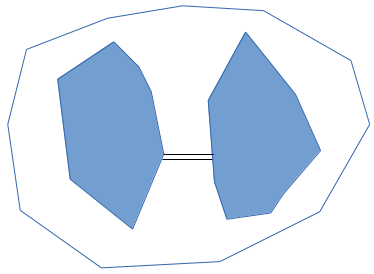
\includegraphics[width=\textwidth]{../picture/bridge-non-conflict.png}
\caption{an acceptable bridge}
\label{fig:bridge-nc}
\end{subfigure}%
~~~~~~~~~~~~~~~~~~~~~~~~~~~~~~~~~~~~~~~~~~~~%add desired spacing between images, blank line to force the
%subfigure to a new line
\begin{subfigure}[b]{0.2\textwidth}
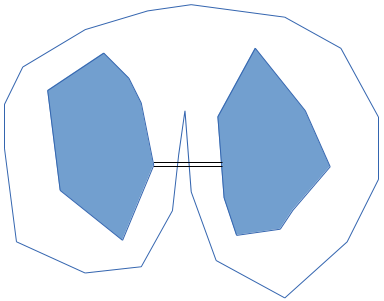
\includegraphics[width=\textwidth]{../picture/bridge-conflict.png}
\caption{a conflicting bridge}
\label{fig:bridge-c}
\end{subfigure}

\caption{Bridges in simple branching case}
\label{fig:bridges}
\end{figure}

For branching problem, Chandrajit et al classified  the approaches into four
methods, shown in Fig. \ref{fig:branches}. The main ideal of solving
the branching problem is converting the one-to-one into a one-to-one
case, Fig. \ref{fig:branch-hull}. shows that a composite contour replaced the branching contours\cite{meyers_surfaces_1992}, so it's converted into a
one-to-one case. apparently, this method will loose details,like
holes. Fig. \ref{fig:branch-bridge} shows that a bridge added between
the branching
contours\cite{barequet_piecewise-linear_1996,christiansen_conversion_1978},
thus reducing to the simple one-to-one case. This method some times
may add a conflicting bridge, or distortion may arise. Recently the
solutions focused on method shown in the Fig. \ref{fig:branch-but}
\ref{fig:branch-middle}, with the developed of the scanning technique,we are
able to reach a slice distance equal to the in-plane resolution. So
interpolate a cure (or a contour) between the slice or in the bottom
slice is no different between visual
effects. Barequet\cite{barequet_reconstruction_2009},
Chandrajit\cite{bajaj_arbitrary_1996},Geiger\cite{geiger_three-dimensional_1993}used
the straight skeleton to do the interpolation, and
Jeong\cite{jeong_b-spline_1999} used the distance map to interpolate
the contours between the slices.
\begin{figure}[ht]
\centering
\begin{subfigure}[b]{0.15\textwidth}
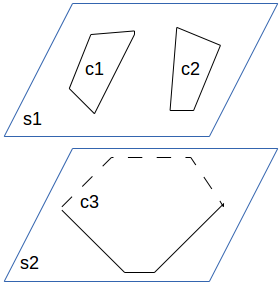
\includegraphics[width=\textwidth]{../picture/branch-contour.png}
\caption{}
\label{fig:branch-contour}
\end{subfigure}%
~%add desired spacing between images, blank line to force the
%subfigure to a new line
\begin{subfigure}[b]{0.1\textwidth}
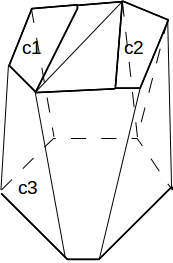
\includegraphics[width=\textwidth]{../picture/branch-hull.png}
\caption{}
\label{fig:branch-hull}
\end{subfigure}
~
\begin{subfigure}[b]{0.1\textwidth}
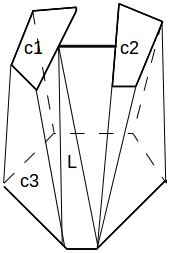
\includegraphics[width=\textwidth]{../picture/branch-bridge.png}
\caption{}
\label{fig:branch-bridge}
\end{subfigure}
~
\begin{subfigure}[b]{0.1\textwidth}
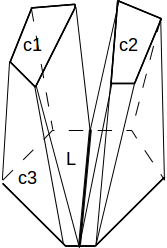
\includegraphics[width=\textwidth]{../picture/branch-but.png}
\caption{}
\label{fig:branch-but}
\end{subfigure}
~
\begin{subfigure}[b]{0.1\textwidth}
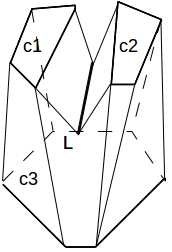
\includegraphics[width=\textwidth]{../picture/branch-middle.png}
\caption{}
\label{fig:branch-middle}
\end{subfigure}


\caption{Different reconstruction for branching contours:(a) branching
contours on adjacent slices;(b)-(e) different surface reconstruction}
\label{fig:branches}
\end{figure}


%\subsection{Our Approach}

%here maybe need more explain

\section{Reconstruction Based on the FFD Matching}
\label{section3}
\subsection{overview of our approach}
To the best of our knowledge, all previous work used the
advancing rule or a set of constraints to get the correspondence, and
it is really hard to deal with the general form, because there are
various types of differences between the adjacent slices. But if the adjacent
slices have high degree of resemblance, almost all the previous works can get a
perfect correspondence, so with this key-point we propose a new
framework which can deform the adjacent contours to have a high degree
of resemblance.
Our proposed framework consists of the following steps,like fig\ref{fig:fluent}:
\begin{description}
\item[$\bullet$]Data acquisition:
\end{description}
Orienting all contours in each slices, and calculate the skeleton for the object.
\begin{description}
\item[$\bullet$]Branching problem:
\end{description}
Locating the branching locate by the skeleton, use the medial axis
projection to subdivide the contour which is the one, in one-to-many
case, and reducing the problem to one-to-one case. See detail in
section \ref{medial axis}.
\begin{description}
\item[$\bullet$]Matching Contour Based on the FFD:
\end{description}
Obtaining the correspondence based on the FFD. See detail in section \ref{ffd}.
\begin{figure}[ht]
\centering
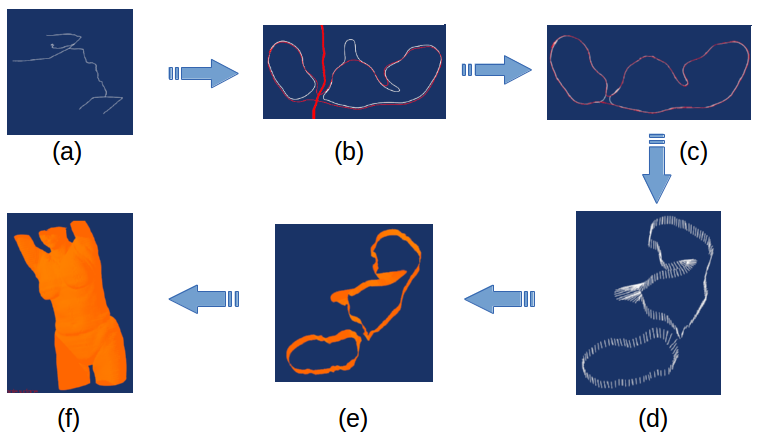
\includegraphics[width=0.5\textwidth]{../picture/fluent.png}
\caption{The basic steps of the reconstruction base on FFD: (a)It's
  the skeleton extract from the contours. (b) A para layers contain
  branches,the contour with white line is upper layer, and the contour
  with red line is lower layer, the bold red line is medial axis of
  the upper layer. (c) The deformation
  based on FFD. (d) The correspondence based on the FFD. (e)(f) The
  surface of the original data}
\label{fig:fluent}
\end{figure}

\subsection{Data Acquisition}
like previous works, we are interesting in the contour's
orientations, since all contours in consistent direction are good for the
triangulation. And the data must consist of a sequence of
slices, since we calculate the skeleton of the object base on the
sequential slices. The skeletal points are the
geometric centers of each contour. the skeleton is used to locate the
branches.

Then distance transform (also know as distance maps) is compute for each slice by determining:

1. The nearest contour curve segment.

2. The distance to the nearest point of each pixel.

The distance transform will be used in the FFD matching and calculation of medial axis.
\subsection{Matching Contour Based on the Free-Form Deformation}
\label{ffd}
In order to get a pair of contours with high degree of resemblance, we
need perform deformation on one of the adjacent contours,local
transformation models can represent pixel-wise deformations that
deform a shape locally and non-rigidly, like optical flow
\cite{paragios_non-rigid_2003}\cite{xu_deformation_2010},Thin Plate
Splines(TPS)\cite{belongie_matching_2001}\cite{roth_registration_2013},
and space deformation techniques such as Free Form
Deformations\cite{huang_shape_2006}. The optical flow and FFD method
can satisfy our demand that transform one contour to another one, both
method can be used according to coarse-to-fine strategy which is more
flexible to applications, FFD is able to implicitly enforce
smoothness constraints, exhibits robustness to noise, and the
recovered deformation field is continuous, preserves shape topology and guarantees a one-to-one mapping, which means a high degree of
resemblance. Other than FFD, the methods based on optical flow is
trying to estimate the motion of the flow filed, and minimize the
object energy. Even with the advanced
regularization and smoothness constraints, the model is not very
suitable for reconstruction since it does not guarantee the
preservation of topology and coherence of a shape after
deformation\cite{paragios_non-rigid_2003}, and it does not
necessarily produce one-to-one correspondences.\cite{huang_shape_2006}.
use the free-form deformation method to get the correspondence.

In this paper we chose the Incremental Free Form Deformation
(IFFD)\cite{huang_shape_2006} to perform the contour's
deformation. Its a B-spline based FFD model which used to minimize a
Sum-of-Squared-Differences(SSD) measure and further recover a dense
local non-rigid registration field.

For a given contour, a regular lattice P overlaid on its surface,the
deformation of the contour is caused by manipulating the Lattice P. The
deformation of the control lattice P consists of the
displacements $\Theta$ as [Eq. \ref{formula:theta}] of
all the control points $\left\{ \mbox{ $\mathbf{p}_{\boldmath{m,n}}$} \right\}$ in the lattice, and from these sparse
displacements $\Theta$, a dense deformation field for every pixel in the
embedding space can be acquired through interpolation using B-spline
function.

\begin{equation}
\label{formula:theta}
\Theta=\left\{\delta \mathbf{p}_{\boldmath{m,n}}\right\}=
\left\{
    \delta p ^{\boldmath{x}}_{\boldmath{m,n}},\delta p^{\boldmath{y}}_{\boldmath{m,n}}
\right\}
;(m,n)\in[1,M] \times [1,N]
\end{equation}

According to the B-splines property, for any pixel $\mathbf{x}$ on the original
shape and its embedding space can represent as [Eq. \ref{formula:original}]
\begin{equation}  
\label{formula:original}
L(\mathbf{x})=\mathbf{x}= \sum\limits_{k=0}^{3}\sum\limits_{l=0}^{3}B_k(u)B_l(v)P^0_{i+k,j+l},\mathbf{x}=\left\{x,y \right\}
\end{equation}

where 

$\bullet$
i=
$\lfloor \frac{x-min_x}{max_x-min_x} \cdot(M-1)\rfloor,
j=\lfloor \frac{y-min_y}{max_y-min_y} \cdot(N-1)  \rfloor$,
this is according to the definition of the cubic B-spline.

$\bullet$
$P^0_{i+k,j+l},\mathbf{x}=\left\{x,y \right\}$ are the control points
in the lattice, $P^0$ means original.

$\bullet$
$B_k(u)(B_l(v))$ are  the $k^{th}$ ($l^{th}$) basis function of the
cubic B-spline.

The new position of pixel x after deformation can be given by

\begin{equation}
\label{formula:deformation}
L(\Theta:\mathbf{x})=\mathbf{x}+\sum\limits_{k=0}^{3}\sum\limits_{l=0}^{3}B_k(u)B_l(v)
\delta P_{i+k,j+l}
\end{equation}

With the definition of deformation, how to deform one contour to
another one is equivalent to finding the control lattice deformation
$\Theta$. For example, we apply these to the upper a layer of the
pair of the contours, and the deformed upper contour coincides with
the lower contour. According to \cite{huang_shape_2006}, we can use
the gradient descent optimization technique to find $\Theta$. The
energy function consist of the data-driven term and smoothness term.

\begin{equation}
\label{formula:data-driven}
E_{data}(\Theta)=\iint\limits_D(\Phi_{u}(\mathbf{x})-\Phi_{l}(L(\Theta:\mathbf{x})))^2d\mathbf{x}
\end{equation}
\begin{equation}
\label{formula:smoothness}
E_{smoothness}(\Theta)=\iint\limits_D\left( \frac{\partial\delta L(\Theta:\mathbf{x})}{\partial x}^2+\frac{\partial\delta L(
\Theta:\mathbf{x})}{\partial y}^2\right) d\mathbf{x}
\end{equation}
\begin{equation}
\label{formual:energy}
\frac{\partial}{\partial \theta} E(\Theta)=\frac{\partial
 }{\partial \theta} E_{data}+\frac{\partial}{\partial \theta} E_{smoothness}
\end{equation}



\begin{figure}[ht]
\centering
\begin{subfigure}[b]{0.25\textwidth}
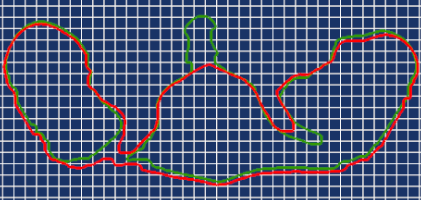
\includegraphics[width=\textwidth]{../picture/FFD_original.png}
\caption{}
\label{fig:FFD_original}
\end{subfigure}
~~~~~~~~~~~~~~~~~~~~~~~~~~~~~~~~~~~~
\begin{subfigure}[b]{0.25\textwidth}
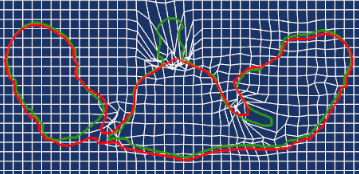
\includegraphics[width=\textwidth]{../picture/FFD_Lattice.png}
\caption{}
\label{fig:FFD_Lattice}
\end{subfigure}

\begin{subfigure}[b]{0.25\textwidth}
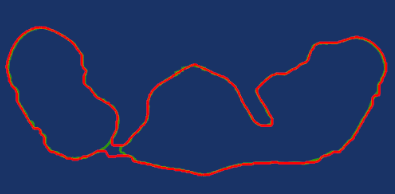
\includegraphics[width=\textwidth]{../picture/FFD_Result.png}
\caption{}
\label{fig:FFD_Result}
\end{subfigure}
\caption{Matching based on the FFD. (a)Final FFD control lattice
  configuration depicting the space warping to achieve local
  registration. (b)Locally deformed upper layer(in green) covered by the lower
  layer(in red)}
\end{figure}

\subsection{Branching Problem}
\label{medial axis}
The FFD technique is only appropriate for no branching case, In the
case of branching, we calculate the medial axis of branching
contours, and project it on to the adjacent contour, thus we reduce
the branching problem to one-to-one case.



region voronoi diagram;medial axis
\section{Results and Discussions}
\label{section4}
\subsection{Capping Region Problem} 
use the energy function to  detect the Capping Region
\subsection{Accurate Reconstruction of Organs}
analyze the accurate of the result of the organ, relation between the
lattice distance and the points intensity.
%% \label{}

%% References
%%
%% Following citation commands can be used in the body text:
%% Usage of \cite is as follows:
%%   \cite{key}         ==>>  [#]
%%   \cite[chap. 2]{key} ==>> [#, chap. 2]
%%

%% References with BibTeX database:

\bibliographystyle{elsarticle-num}
\bibliography{reference}

%% Authors are advised to use a BibTeX database file for their reference list.
%% The provided style file elsarticle-num.bst formats references in the required Procedia style

%% For references without a BibTeX database:

% \begin{thebibliography}{00}

%% \bibitem must have the following form:
%%   \bibitem{key}...
%%

% \bibitem{}

% \end{thebibliography}

\end{document}

%%
%% End of file `ecrc-template.tex'. 
% Local Variables:
% zotero-collection: #("0" 0 1 (name "*ALL*"))
% End:
